\documentclass[11pt, twoside]{article}

\oddsidemargin=0in
\evensidemargin=0in
\textwidth=6.3in
\topmargin=-0.5in
\textheight=9in

\usepackage{amsmath, amsfonts}
\usepackage{graphicx}
\usepackage{epstopdf}
\usepackage{subfigure}
\usepackage{multicol}
\usepackage{subfig}
\usepackage{color}
\usepackage{enumitem}
\usepackage{float}     % Using this package along with the placement specifier
                       % [H] makes figures appear at that exact position in the
                       % file.
\allowdisplaybreaks[4]

\title{
	18-752 Course project report\\
	Internet Traffic Dataset: Hidden Markov Model
}
\date{}
\author{
	Praveen Venkatesh\\
	Department of Electrical and Computer Engineering\\
	\texttt{praveen1@andrew.cmu.edu}
}

\begin{document}

\maketitle

\section{The dataset and project goals}

The internet traffic dataset that I used for this project was aquired from [1]. It consists of one hour's worth of internet traffic between the Lawrence Berkeley laboratory and the rest of the world.

This data has been previously used to show that internet traffic data is not Poisson, that it is very bursty, and needs more sophisticated models [2].

The goal of this project is to show that a simple Poisson model \emph{is} in fact a bad fit, and to find a better fit using a Hidden Markov Model.

\section{Data histograms}

\subsection{Non-Poisson data}

A plot of the data reveals its extremely bursty nature, as shown in Figure~\ref{fig:data}.
\begin{figure}[h!]
	\centering
	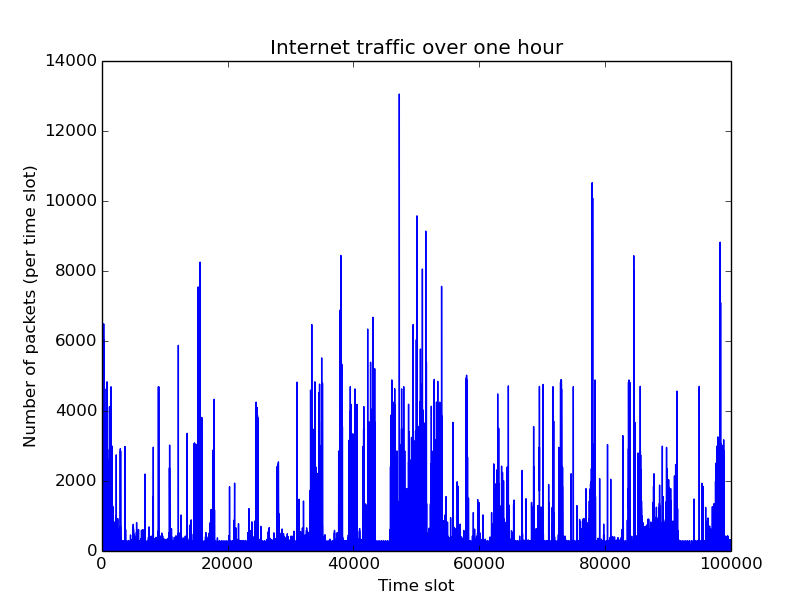
\includegraphics[scale = 0.7]{data}
	\caption{Plot of the data: number of packets per time-slot over time slots}
	\label{fig:data}
\end{figure}

To understand whether or not the data has some underlying structure, we look at histograms of the packet counts. The first such plot (not shown here) reveals that there is an extremely heavy concentration of packet numbers at the lower range of packet sizes. This is because in nearly 80\% of the time slots, there were no packets. Plotting the histogram in only non-zero time slots still reveals a heavy concentration towards lower packet sizes. In order to capture and depict the full range of packet sizes and their frequencies, multiple histograms were deemed required. These are shown in Figure~\ref{fig:packet-histograms}.

\begin{figure}[h!]
	\centering
	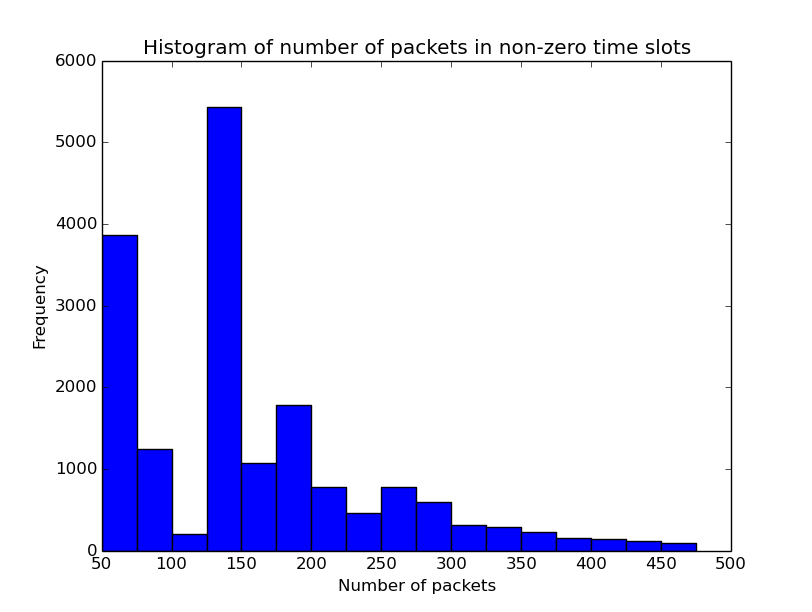
\includegraphics[scale = 0.35]{packet-hist-coarse}
	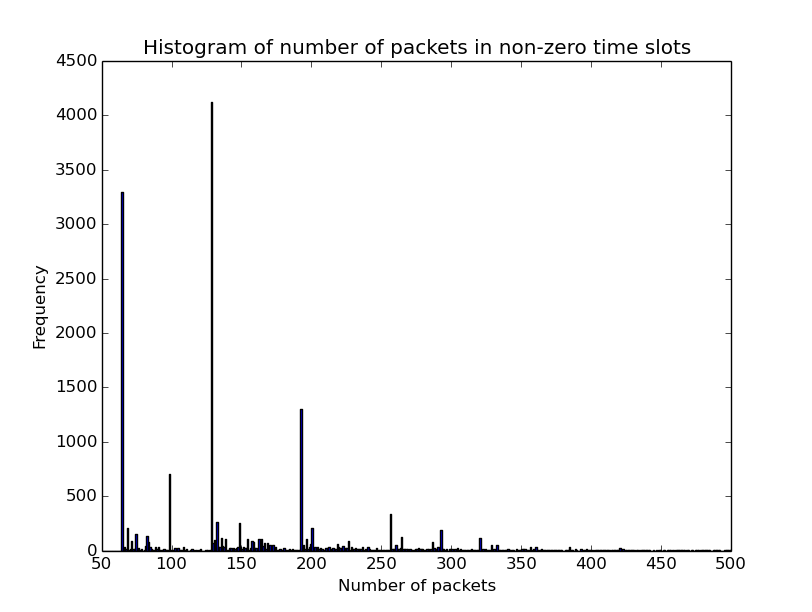
\includegraphics[scale = 0.35]{packet-hist-fine}
	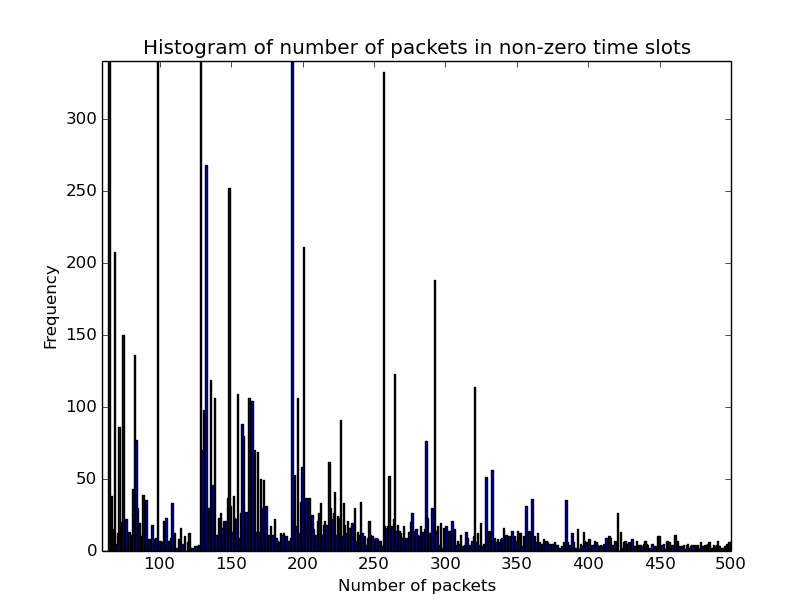
\includegraphics[scale = 0.35]{packet-hist-fine-zoom}
	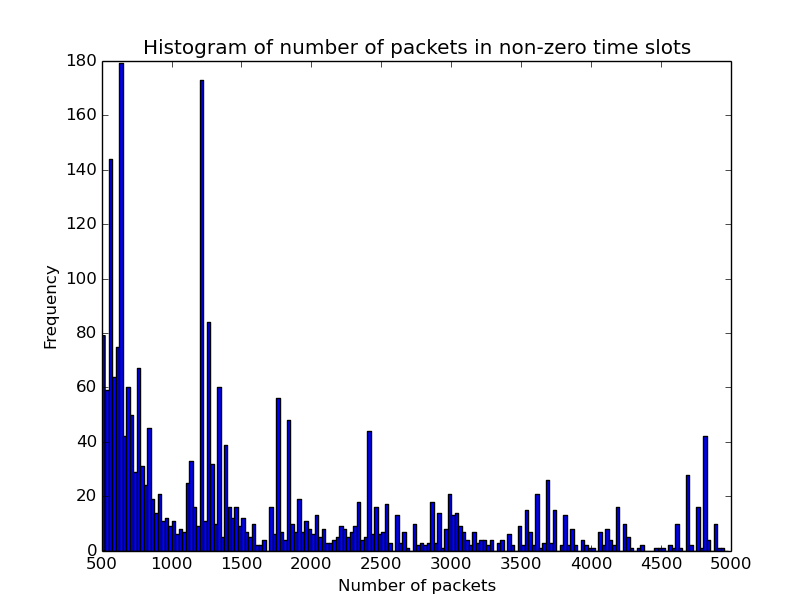
\includegraphics[scale = 0.35]{packet-hist-500-5000}
	\caption{Packet histograms for different packet-size ranges. Top left, top right and bottom left are over the same size range. Top left has large bin-sizes. Decreasing bin-size reveals a high degree of irregularity, with most of the frequency concentrated in very few packet sizes. Bottom left shows a zoomed-in version of the plot at the top right, revealing some underlying structure, outside of the high-frequency outliers. Bottom right shows the rest of the packet size range.}
	\label{fig:packet-histograms}
\end{figure}

It is very obvious from these histograms that the packet size distribution cannot be captured using a simple distribution, such as a Poisson distribution. A mixture model might be able to fit the data, however it will not capture any temporal variation of packet sizes over time. Hence, we use a Hidden Markov model that tries to capture both the packet-size distribution and its evolution over time.

\subsection{Bursts and burst statistics}

Packet sizes have been seen to be non-Poisson. Further, packet inter-arrival times are said not to follow a Poisson distribution. We do not have the capability to check whether or not packets arrived as a Poisson point process from the raw data, since it only has packet counts in discrete time slots. So to demonstrate, we aggregate packets into ``bursts''. A burst is defined by a set of packets that have at least a predefined \verb+num_zeros+ number of zeros before and after it. The start time of the burst is considered to be the burst arrival time. Using this, we compute burst inter-arrival times, for different values of \verb+num_zeros+.

For small values of \verb+num_zeros+, the exponential fit becomes a poor one - it underestimates the distribution, especially at large inter-arrival times. This is a result of so-called ``long-range dependency'', which means that the decay of statistical dependence is slower than exponential. This is characteristic of internet traffic. The Pareto distribution (which is a heavy-tailed distribution, capable of capturing such long-range dependencies) is actually a better fit, as is evident on the log scale plots of Figure~\ref{fig:burst-statistics}.
\begin{figure}[h!]
	\centering
	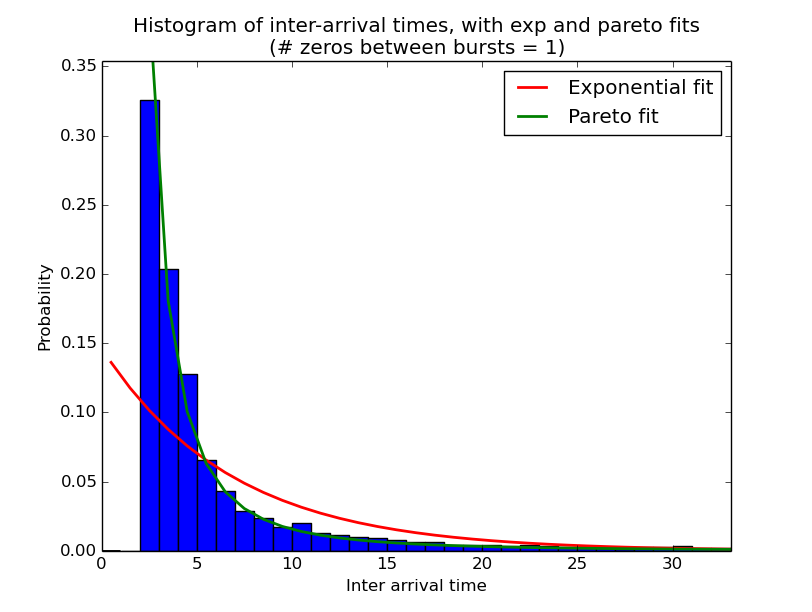
\includegraphics[scale = 0.35]{ipt-1}
	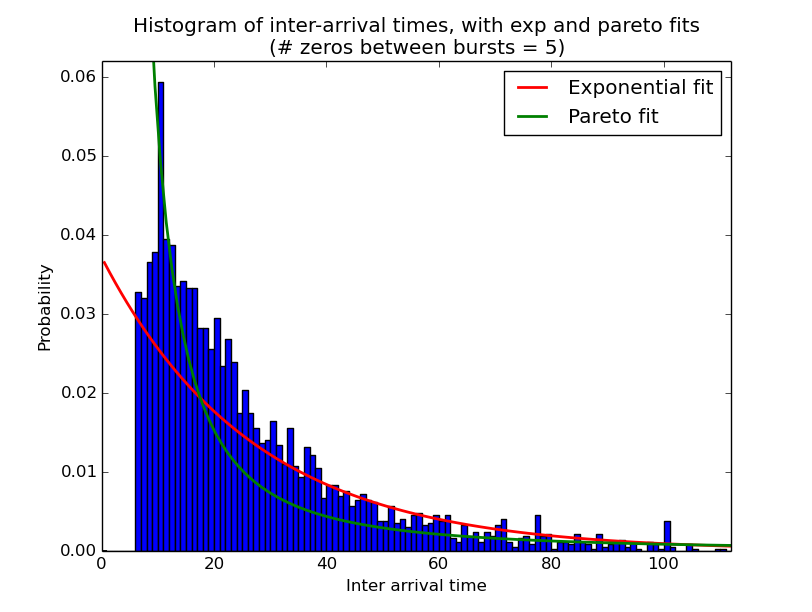
\includegraphics[scale = 0.35]{ipt-5}
	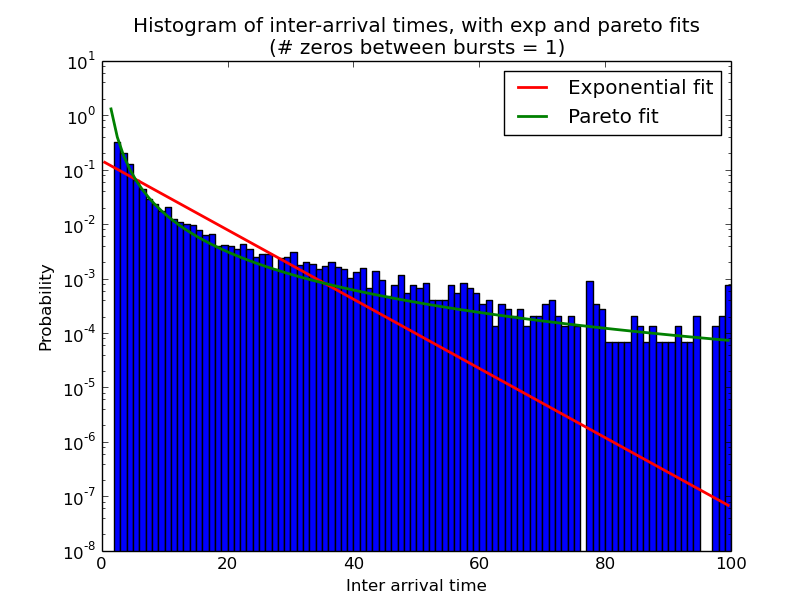
\includegraphics[scale = 0.35]{ipt-1-log}
	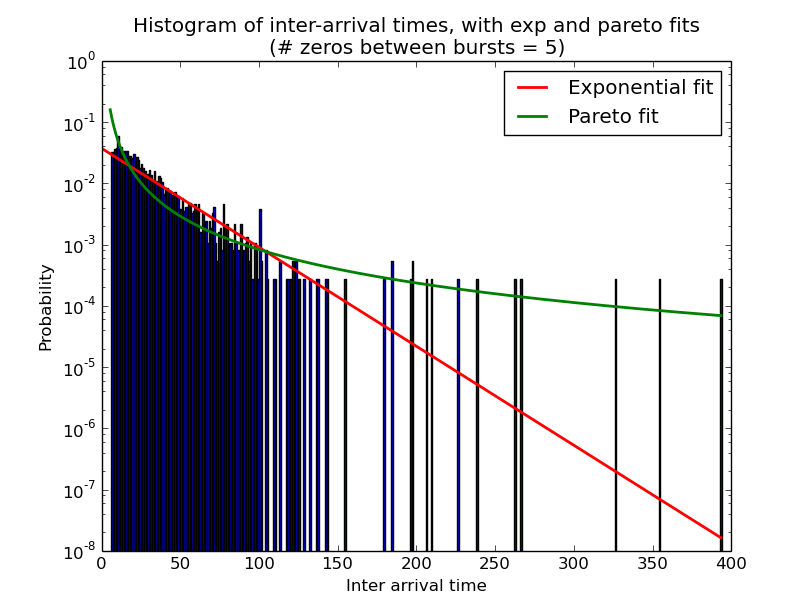
\includegraphics[scale = 0.35]{ipt-5-log}
	\caption{Histograms of burst inter-arrival times with exponential and pareto fits. Top-left: \texttt{num\_zeros}=1; Top-right: \texttt{num\_zeros}=5; Bottom-left: \texttt{num\_zeros}=1, log-scale; Bottom-right: \texttt{num\_zeros}=5, log-scale. The exponential fit does relatively better for the case where \texttt{num\_zeros}=5, because most of the data is concetrated in the linear regime, but the pareto fit still out-performs it in general}
	\label{fig:burst-statistics}
\end{figure}

\section{The Hidden Markov Model}

In a Hidden Markov Model, the assumption is that there is some underlying set of states that system moves between. In each state, the system output is determined by some state-dependent paramters. In our model, we assume that the system output is a Poisson random variable, with a state-dependent mean.

The model is determined by three vector parameters - the initial probability distribution on the set of states (which decides which state the Markov chain starts in), the probability transition matrix (which decides the probabilities of transitioning from one state to another) and the parameters that decide the output at each state. We label these parameters as $\theta = (\underline{q}, A, \underline{\mu})$ respectively.

There are several things that one can do with this kind of model [3]:
\begin{itemize}
	\item \emph{Evaluation}: Given an HMM $\theta$, and a sequence of observations (outputs) $\{y_t\}$, we can compute the probability of seeing this set of outputs. This uses the so-called forward-backward algorithm to efficiently compute these values.
	\item \emph{Reconstruction}: Given an HMM $\theta$ and a sequence of observations $\{y_t\}$, we can estimate the states $\{x_t\}$ that the system went through to give these outputs. This can be done using the Viterbi algorithm.
	\item \emph{Learning}: Given an output sequence $\{y_t\}$, we can find the HMM $\theta$ that maximizes the likelihood of seeing this output. This uses a special case of the Expectation-Maximization algorith, called the Baum-Welch algorithm.
\end{itemize}

In this project, we take up all three tasks - learning an HMM model for the given dataset, which involves evaluation as a part of the algorithm. We also undertake reconstruction, but we use an intermediate step of the Baum-Welch algorithm to find the most likely states, given the output sequence and the current estimate of the chain.

\subsection{Learning the HMM parameters}

Learning the HMM parameters follows an iterative procedure. We first assume some initial HMM parameters, and compute the likelihood function. We then try to maximize the liekelihood function over the parameter space [4]. This effectively takes the form of the algorithm described below.

We start by computing the forward and backward probabilities. The forward probability $\alpha_i(t)$ is the probability of arriving at the state $i$ at time $t$, and seeing observations $y_1$ to $y_t$ en route, given the HMM $\theta$. The backward probability $\beta_i(t)$ is the probability of seeing the future observations $y_{t+1}, \ldots, y_T$, given that you start in state $i$ at time $t$.

\begin{align*}
	\alpha_i(t) &= \mathbb{P}(Y_1=y_1, \ldots, Y_t=y_t, X_t=i | \theta) \\
	\beta_i(t) &= \mathbb{P}(Y_{t+1}=y_{t+1}, \ldots, Y_T=y_T | X_t=i, \theta)
\end{align*}

These can be computed iteratively. If $b_i(y)$ is the probability of seeing the output $y$ in state $i$ (i.e.\ $b_i(y) = \frac{1}{y!} e^{-\mu_i} \mu_i^y$), then we have:
\begin{align*}
	\alpha_i(1) &= q_i b_i(y_1) & \forall &\; i = 1, \ldots, N \\
	\alpha_j(t+1) &= b_i(y_{t+1}) \sum_{i=1}^{N} \alpha_i(t) A_{ij} & \forall &\; t = 2, \ldots, T \\
	\beta_i(T) &= 1 & \forall &\; i = 1, \ldots, N \\
	\beta_i(t) &= \sum_{i=1}^N A_{ij} b_j(t+1) \beta_j(t+1) & \forall &\; t = 1, \ldots, T-1
\end{align*}

We then compute the intermediate variables: $\gamma_i(t)$, the probability of being in state $i$ at time $t$, given the observations $y_1, \ldots y_T$ and the HMM $\theta$, and $\xi_{ij}(t)$, the probability of transitioning from state $i$ to state $j$ in going from time step $t$ to $t+1$, given the observations and the HMM.

These are derived using Bayes' rule, as follows:
\begin{align*}
	\gamma_i(t) &= \mathbb{P}(X_t = i | Y_1=y_1, \ldots, Y_T=y_T, \theta) \\
	            &= \frac{\mathbb{P}(X_t = i, Y_1=y_1, \ldots, Y_T=y_T | \theta)}{\mathbb{P}(Y_1=y_1, \ldots, Y_T=y_T | \theta)} \\
	            &= \frac{\mathbb{P}(X_t = i, Y_1=y_1, \ldots, Y_t=y_t | \theta) \mathbb{P}(Y_{t+1}=y_{t+1}, \ldots, Y_T=y_T | \theta)}{\mathbb{P}(Y_1=y_1, \ldots, Y_T=y_T | \theta)} \\
	            &= \frac{\alpha_i(t) \beta_i(t)}{\sum_{j=0}^N \alpha_j(t) \beta_j(t)} \; \; \forall \; t = 1, \ldots, T
\end{align*}
where for the second-last step, we have relied on the Markov-ness of the Markov chain, which implies that the state of the Markov chain captures everything about the history of the process.

A similar derivation for $\xi$ yields
\begin{align*}
	\xi_{ij}(t) &= \mathbb{P}(X_t=i, X_{t+1}=j | Y_1=y_1, \ldots, Y_T=y_T, \theta) \\
	            &= \frac{\alpha_i(t) A_{ij} b_j(t) \beta_j(t+1)}{\sum_{k,l=1}^N \alpha_k(t) A_{kl} b_l(t) \beta_l(t+1)} \; \; \forall \; t = 1, \ldots, T-1
\end{align*}

We can then update the HMM parameters:
\begin{align*}
	\hat{q}_i &= \gamma_i(1) \\
	\hat{ A}_{ij} &= \frac{\sum_{t=1}^{T-1} \xi_{ij}(t)}{\sum_{t=1}^{T-1} \gamma_i(t)} \\
	\hat{\mu}_i &= \frac{\sum_{t=1}^T y_t \gamma_i(t)}{\sum_{t=1}^{T} \gamma_i(t)}
\end{align*}
These become the new set of parameters for the next iteration of the Baum-Welch algorithm.

\section{Results}

We fit an HMM with four states to the non-zero component of the data, starting with the initial parameters:
\begin{align*}
	\underline{q} &= [ \begin{array}{cccc}
	0.25 & 0.25 & 0.25 & 0.25 \end{array} ] \\
	A &= \left[ \begin{array}{cccc}
	0.25 & 0.25 & 0.25 & 0.25 \\
	0.25 & 0.25 & 0.25 & 0.25 \\
	0.25 & 0.25 & 0.25 & 0.25 \\
	0.25 & 0.25 & 0.25 & 0.25 \end{array} \right] \\
	\underline{\mu} &= [ \begin{array}{cccc}
	1 & 100 & 1000 & 10000 \end{array} ] \\
\end{align*}

We show in figure~\ref{fig:mu-convergence} the convergence of the values of the parameter $\underline{\mu}$ over the iterations of this algorithm.
\begin{figure}[h!]
	\centering
	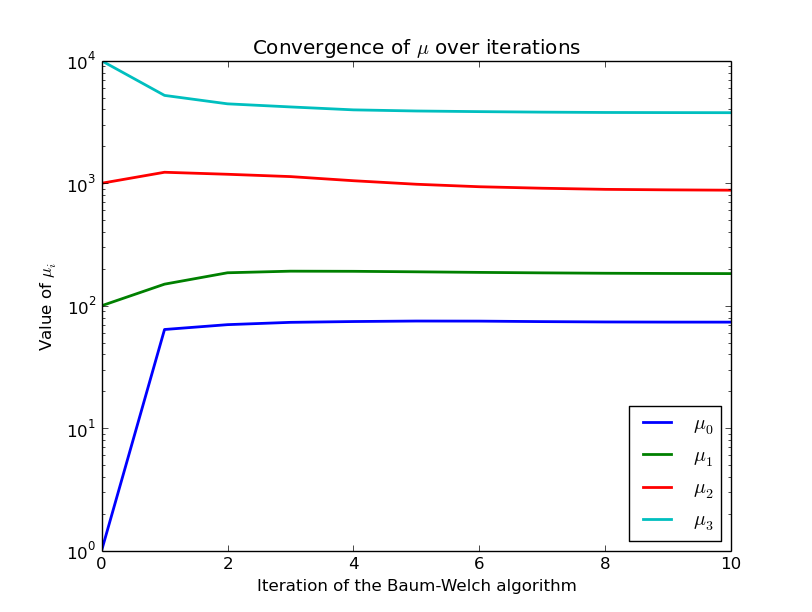
\includegraphics[scale = 0.4]{mu-convergence}
	\caption{Plot of the data coloured by state}
	\label{fig:mu-convergence}
\end{figure}

The final parameters are approximately
\begin{align*}
	\underline{q} &= [ \begin{array}{cccc}
	1 & 0 & 0 & 0 \end{array} ] \\
	A &= \left[ \begin{array}{cccc}
	0.722 & 0.264 & 2 \times 10^{-6} & 0.014 \\
	0.586 & 0.390 & 8.6 \times 10^{-6} & 0.024 \\
	0.283 &  0.428 & 3.6 \times 10^{-5} & 0.290 \\
	0.074 &  0.036 & 3.6 \times 10^{-5} & 0.889 \end{array} \right] \\
	\underline{\mu} &= [ \begin{array}{cccc}
	108 & 281 & 1133 & 3682 \end{array} ] \\
\end{align*}

Using the final value of $\gamma_i(t)$, we compute the most likely state as
\begin{equation*}
	\hat{x}_t = \text{argmax}_i \gamma_i(t)
\end{equation*}

This method yields a set of states, but does not provide a smooth transition from states corresponding to small $\mu$ to states corresponding to large $\mu$. Furthermore, there is a high tendency to keep switching states. The model essentially goes to the most suitable state for the given output, without taking neighbouring values into account. In order to fix this, we impose some restrictions on the probability transition matrix $A$. We make it a banded matrix, with only the diagonal and first off-diagonal elements being non-zero. We also add some value to its diagonal elements and re-normalize along the rows, so that there is an increased chance of staying in the same state. Finally, we start with the transition matrix
\begin{equation*}
	A = \left[ \begin{array}{cccc}
	0.5 & 0.5 & 0 & 0 \\
	0.3 & 0.4 & 0.3 & 0 \\
	0 & 0.3 & 0.4 & 0.3 \\
	0 & 0 & 0.5 & 0.5 \end{array} \right]
\end{equation*}

We impose these restrictions at each iteration of the parameter-update step. This leads to smoother transitions, as shown in figure~\ref{fig:state-transitions}.
\begin{figure}[h!]
	\centering
	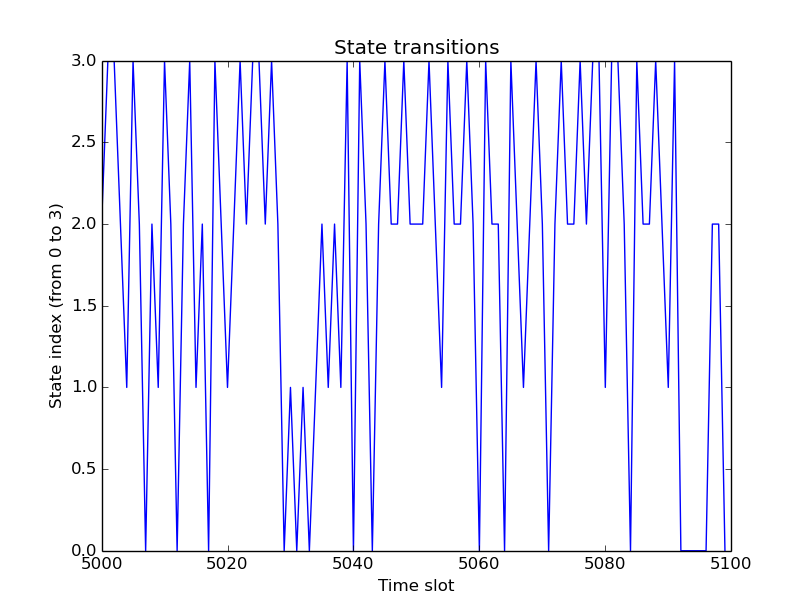
\includegraphics[scale = 0.35]{state-transitions-rough}
	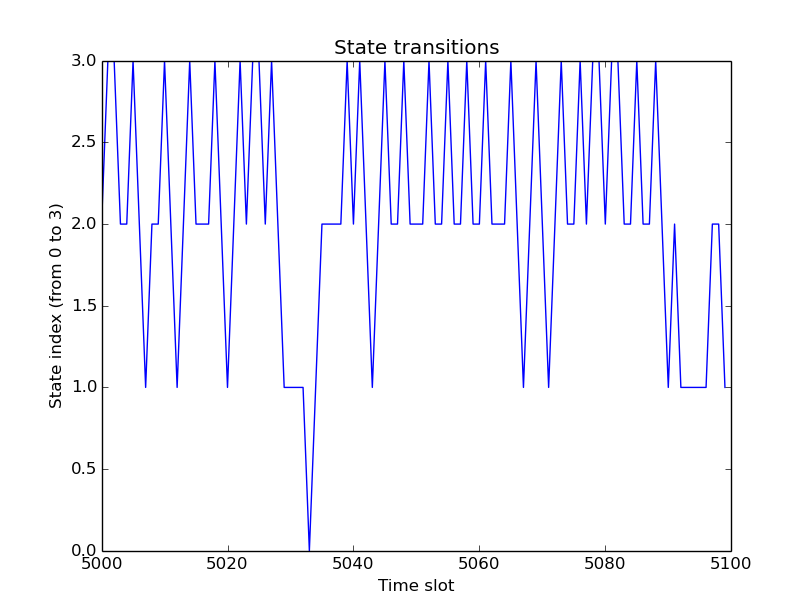
\includegraphics[scale = 0.35]{state-transitions-smooth}
	\caption{Plot of state transitions in a short time window; left: before applying the restriction on the probability transition matrix, right: with the smoothness restriction in place. In the latter case, the diagonal values of $A$ were forced to be more that 0.5}
	\label{fig:state-transitions}
\end{figure}

After colouring in the states, the data looks as shown in Figure~\ref{fig:data-with-states}.
\begin{figure}[h!]
	\centering
	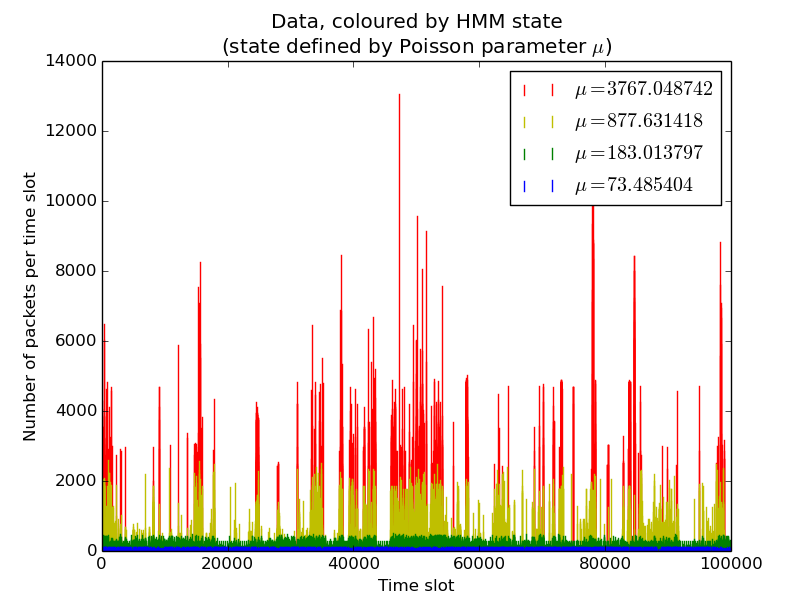
\includegraphics[scale = 0.7]{data-with-states}
	\caption{Plot of the data coloured by state}
	\label{fig:data-with-states}
\end{figure}

\subsection{Numerical difficulties}

Several numerical difficulties were encountered due to the large packet counts in the data and due to the inherent nature of the Baum-Welch algorithm:
\begin{enumerate}
	\item \emph{Computation of $b_i(y)$}: The Poisson probability $b_i(y)$ could not be computed using the direct formula for the Poisson distribution, as $\mu_i^y$ and $y!$ were both very large quantities, since $y \sim 10^3$. Instead, we used $b_i(y) = \exp( -\mu_i + y \log(\mu_i) - \log(y!) )$, where $\log(y!)$ was computed using the \verb+gammaln+ special function.
	\item \emph{Normalization of small values of $\alpha$ and $\beta$}: The Baum-Welch algorithm can yield very small values for $\alpha$ and $\beta$. Inability to express these quantities produces \verb+nan+s when computing $\gamma$ and $\xi$. Therefore, we normalize $\alpha$ and $\beta$ as suggested in [4]. Also, we move to using quadruple precision.
\end{enumerate}

\section*{References}

\begin{enumerate}[label=(\arabic*)]
	\item \texttt{ftp://ftp.esat.kuleuven.be/pub/SISTA/data/timeseries/internet traffic.dat.gz}
	\item V.\ Paxson and S.\ Floyd, ``Wide-area traffic: The failure of Poisson modeling'', \emph{IEEE/ACM Transactions on Networking}, 1995
	\item Alberto Dainotti et.\ al., ``Internet traffic modeling by means of Hidden Markov Models'', \emph{Computer Networks}, 2008, Vol.\ 52, pp. 2645--2662
	\item D.\ J.\ Daley, D.\ Vere-Jones, ``An Introduction to the Theory of Point Processes: Volume II, 2nd Ed.'', \emph{Springer Publications}, Chapter 10: Point Processes Defined by Markov Chains.
\end{enumerate}

\end{document}
